\chapter{Experiments} % Experimental Study of Watershed Weighting Strategies}
\label{Chapter5}
The majority of our experiments focuses on weighting the watershed locations. That corresponds to the \textbf{Structured voting (SV)} stage of the pipeline that we propose for the task of going from edges to contours: SE-SV-UCM.

\textbf{Dataset:} For the evaluation of our segmentation results we work on the Berkeley Segmentation Data Set (BSDS500)~\cite{Arbelaez11}. Since its introduction in 2001, it has by now become a standard dataset for both the task of edge detection as well as that of image segmentation.

\textbf{Benchmark:} We report results on the benchmark of~\cite{Galasso13} which can evaluate segmentation hierarchies against given ground-truth segmentations. It demonstrates the tradeoff between an oversegmentation and a more accurate object-centric segmentation.

\textbf{Watershed weighting strategy:} The Structured voting requires a choice of a watershed weighting strategy. The purpose of the weighting is associating a score with each of the watershed locations pixels. That score must faithfully reflect the strength of the underlying boundary. So we want to evaluate how good is the boundary evidence presented by the most likely segmentation determined by the structured forest. The first aspect of it is making the structured forest patch and the watershed locations patch comparable. The watershed patch is an oversegmentation, and in this sense, contains much more information, not exclusively about the location of the boundary that we would like to evaluate. So we strive to simplify the watershed patch, keeping only important information about it - the shape of the boundary under consideration, or the constitution of the segmentation in the patch. Such a simplification in the context of our algorithm we call ``watershed patch transformation''. The second particular to a watershed weighting strategy is the choice of scoring function. We view the task as a segmentation benchmark problem, where one of the patches is the ground truth segmentation, and the other - the segmentation under test. We analyse and apply a selection of boundary- and region- based metrics.

In the rest of the chapter we briefly describe the dataset and evaluation metrics used to help understand the experiments. Afterwards, we give a detailed account of ours most important experiments and the conclusions we draw based on them.

% \textbf{Oracle} To evaluate the correctness of our weighting strategies, we've implemented an oracle for our pipeline. The question we wanted to answer is ``how well could we perform segmentation in the presence of perfect information?'' Our Structured voting lends itself easily to such an experiment using the ground truth segmentation. When scoring a given pixel on the watershed regions boundary, we use a ground truth segmentation patch, rather than the most likely segmentation learnt by the structured forest. The second patch, as in the regular experiments, comes from the watershed locations image, taken for the same pixel location.

\section{Evaluation setup}
\subsection{Dataset}
The Berkeley Segmentation Data Set (BSDS), introduced in~\cite{Martin01}, is a large dataset of natural images that have been manually segmented by multiple participants. It, therefore, provides the ground truth label for each pixel as being on- or off-boundary. Initially the dataset featured 300 images (BSDS300). It was later extended - in BSDS500~\cite{Arbelaez11} the original 300 images are used for training (200) and validation (100), and 200 new human-annotated images are added for testing. Again, each image is segmented by different subjects.

% TODO put in tabular
\begin{figure}[ht!]
 \centering
 \subfigure[Input image]{%
 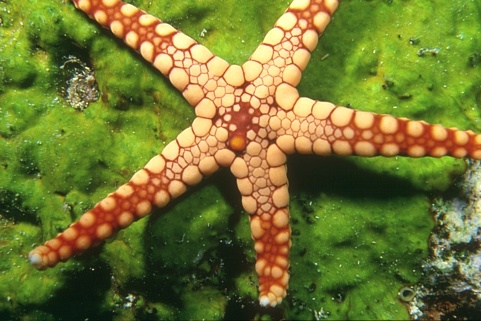
\includegraphics[width=0.3\textwidth]{images/examples/starfish/starfish.png}
 }
 \subfigure[Segmentation by subject 1]{%
 
\includegraphics[width=0.3\textwidth]{images/examples/starfish/starfish_segm_coarse.png}
 }
 \subfigure[Boundaries by subject 1]{%
 
\includegraphics[width=0.3\textwidth,frame]{images/examples/starfish/starfish_bdry_coarse.png}
 }
 \subfigure[Segmentation subject 2]{%
 
\includegraphics[width=0.3\textwidth]{images/examples/starfish/starfish_segm_detail.png}
 }
 \subfigure[Boundaries subject 2]{%
 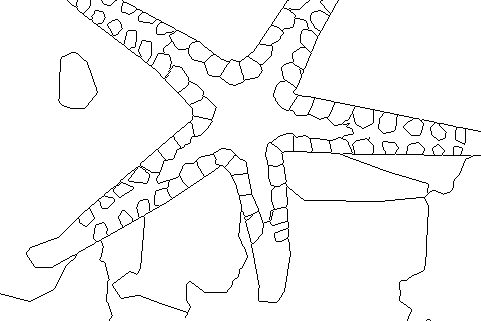
\includegraphics[width=0.3\textwidth,frame]{images/examples/starfish/starfish_bdry_detail.png}
 }
 \caption{Image from the validation subset of~\cite{BSDS500resources} and two of its annotations - human-marked boundaries and their corresponding segmentation reconstructions.}
\end{figure}

\subsection{Metrics}
%\textbf{Two evaluation metrics - BPR and VPR:}
The benchmark that we use provides, among others, two precision-recall metrics - a boundary and a region oriented one.

\subsubsection*{BPR}
The Boundary Precision-Recall (BPR)~\cite{Arbelaez11} is a boundary-based metric and emphasises the correct placement of image edges. Section~\ref{BPR-maths} gives mathematical account on the metric and its properties. In case of segmentation, BPR is a good indicator of the localisation of the region boundaries.

A difference in the score of a single region boundary pixel should not greatly affect the edge detector output. Therefore, it correctly has only a small impact on the BPR metric. For the task of image segmentation however, a change in a single pixel could result in merging neighbouring regions. In the hierarchical image segmentation framework, that means multiple levels of the segmentations hierarchy would change. So a rigorous image segmentation benchmark metric should not be oblivious to such changes.

\subsubsection*{VPR}
To address the above issue, the other metric that we report is the Volume Precision-Recall (VPR) introduced by Galasso \etal~\cite{Galasso13} to evaluate the accuracy of video segmentation algorithms. For images (or video still frames) the metric is a region-based metric, measuring the size of the regions and the overlap between the ground truth segmentation regions and the segmentation regions produced by the algorithm under test. See~\ref{VPR-maths} for the formulae and discussion on the necessity of % need for 
normalisation when evaluating segmentations.

% \section{Weighting strategies} % Exploration of the Space of Weighting Strategies}
% \section{Oracle} %  - Experiments with Ground Truth}
% \subsection{Oracle definition} % description}
% \subsection{Ranking of oracles}
% % \subsubsection{Confirms Correct Weighting Strategies}
% % \subsubsection{Failure Cases}


\textbf{Experiments}
\begin{enumerate}
\item{\bf From edges to contours - a proof of concept:}
 We apply a vanilla watershed algorithm~\cite{beucher1992morphological,najman1996geodesic,PINKlibrary} to the SE output. The result is a single segmentation. % Since the watershed segmentation is a seed-growing segmentation
 In our benchmark plots the outcome of the experiment is not a Precision-Recall curve, but a single dot, indicative of the model error. Since the watershed transformation provides an oversegmentation of the image, the dot is located in the high-recall, low-precision range on the BPR plot.
 
 Note that the SE algorithm implements non-maximum suppression on the edge detection output to provide thinned edges. Non-maximum suppression is a method first introduced as a means of reducing thick edge responses to thin lines for the task of edge detection in greyscale images~\cite{rosenfeld1976digital}. Non-maximum suppression considers only the maxima in the gradient direction. As a consequence, the final output of the SE often has only single regional minimum. In the presence of a unique lake, the watershed is empty. To circumvent this problem, we use the SE detector \textit{before non-maxima suppression} as topographic surface for the flooding.

\item{\bf Baseline: SE-UCM}
 As a baseline, we create a hierarchy of segmentations on top of the SE detector result. This is in the spirit of~\cite{arbelaez2006boundary} who use the edge detector of Martin, Fowlkes, and Malik (MFM)~\cite{martin2004learning}.
 We observe the problem of strong edges ``bleeding'' into non-salient ones, despite lack of good local boundary evidence, as on the tikis examples (see Figure~\ref{fig:SE-UCM-tikis-bleeding}\subref{fig:SE-UCM-tikis-bleeding-sub2}) between the heads of the middle and right statues.

 \begin{figure}[ht!]
 \centering
 \subfigure[Input image]{%
  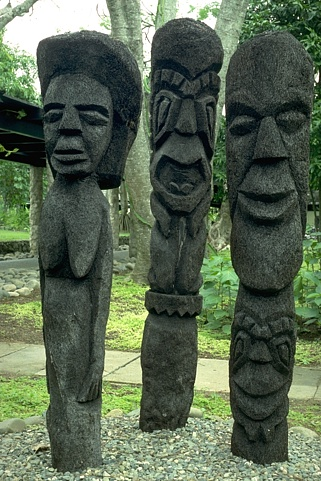
\includegraphics[width=0.3\textwidth]{images/examples/tikis/tikis.jpg}
 }
 \subfigure[SE-UCM result - hierarchical segmentation,frame]{%
  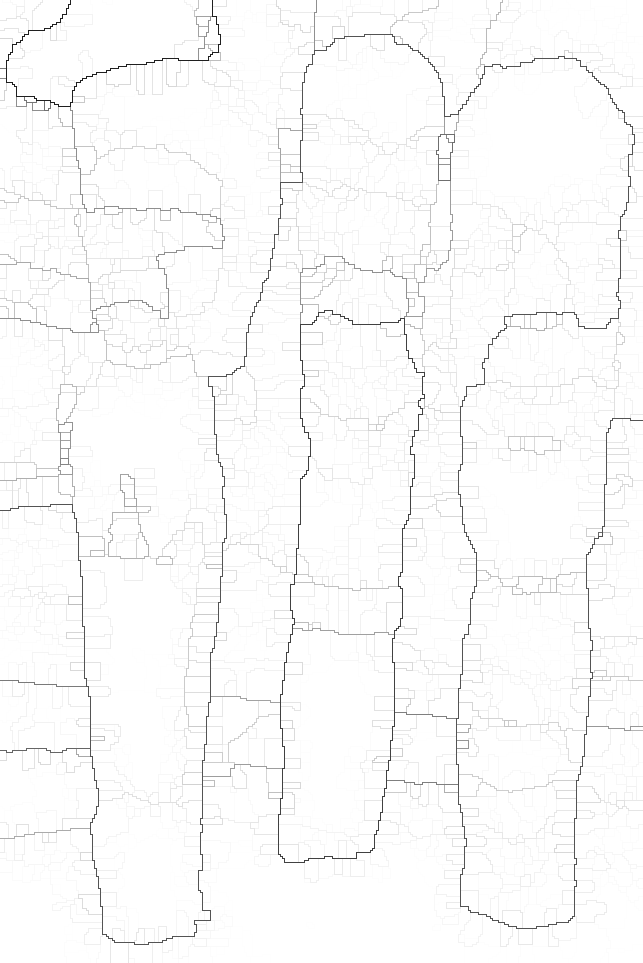
\includegraphics[width=0.3\textwidth,frame]{images/examples/tikis/SE-UCM-tikis-ucm-problem.png}
  \label{fig:SE-UCM-tikis-bleeding-sub2}
 }
 \caption{Image from the validation subset of~\cite{BSDS500resources}. Notice how unimportant horizontal edges between the statues heads are wrongly up-voted due to strong vertical boundary - the statues outline, in their vicinity.}
 \label{fig:SE-UCM-tikis-bleeding}
 \end{figure}
 % BPR edge detector MFM 0.65, MFM-UCM 0.67 ; SE 0.70, % SE_no_nms_single_scale_repeat
 % SE-UCM 0.70

\item{\bf SE+sPb-UCM:} This experiment shows us that globalisation could easily be introduced to our method. Here we use the same affinity matrix as the spectral Pb of Arbel\'aez \etal~\cite{Arbelaez11}. Extending our algorithm to adopt a globalisation step could be beneficial, since it could pick up on improvements in the realm of spectral clustering, as for example spectral reduction~\cite{Galasso14}. % check the plots, check MCG paper - they did exactly this

\item{\bf First Structured voting - superpixels and Rand Index:} We leave the watershed patch to be an oversegmentation, which in fact it is. The output of the watershed transform that we use has explicit the boundaries between segments, which would hinder a region-based metric. Therefore, we transform a watershed patch to have implicit segment boundaries - the locations of transition between differently labelled segments. The patches from the decision forest already constitute segmentation labelling with implicit segment boundaries. That, of course, is due to the fact that the structured forest patches are taken unmodified from the ground truth segmentations of the training subset of BSDS500, which has a ``labelling with implicit segment boundaries'' format. We conduct the comparison between watershed and a tree leaf patch using as a scoring function:

 \begin{itemize}
  \item{\bf Rand Index (RI):} a count of the number of pairs of locations that belong to the same segment in both patches. For a $16\times16$ segmentation patch, that means $32 640$ pairs of locations.
  \item{\bf Rand Index Monte Carlo (RIMC):} ours randomised subsample version of RI, which takes only a fraction $\rho$ of the pairs of locations into consideration. We experience no reduction in performance \wrt RI for a fraction as small as $\rho\approx\frac{1}{128}$, \ie, 256 out of the $32 640$ possible pairs of locations in a $16 \times 16$ patch. This scoring function is inspired from the way features are subsampled to introduce randomness when training a decision tree in~\cite{DollarICCV13edges,Dollar2013toolbox}.
 \end{itemize}

 The above experiments (both having a result of $F=0.55$ on BPR) led us to two conclusions. First, we need to have a closer look into the properties of our \textbf{scoring functions}. Section~\ref{boundary-and-region-metrics-maths} of the previous chapter gives mathematical formulae and a detailed explanation on the metrics we considered for this task. Second, a \textbf{simplification of the watershed patch} is desirable, due to the discrepancy %mismatch between 
 in makeup %constitution
 of watershed and decision tree patches.

\item{\bf Na\"{\i}ve greedy merge of watershed patch:} We first address the second of our conclusions from the previous experiment. We merge segments in the watershed patch according to each of the $T$ leaf patches (where $T$ is the number of trees in the decision forest). Thus we end up with $T$ distinct ``merged'' watershed patches. This approach seems to be too greedy, however. The watershed patch eventually becomes overly adapted to the tree leaf patch it is being compared to. As a consequence, this watershed transformation is not discriminative enough.

 \begin{itemize}
  \item{\bf Fair greedy merge:} To remedy this shortcoming of the na\"{\i}ve greedy merge, we introduce what we call ``fairness'' in the greedy merge approach. As described previously, we cast votes only on the watershed locations. That means, the patches that we consider contain a potential boundary location at their central pixel. It is the strength of this boundary that we strive to quantify. We enforce the greedy merge to respect a boundary-at-centre-location condition by preventing excessive merge of the segments around the central pixel of the patch.
  % TODO image of the patches
 \end{itemize}

Figure~\ref{fig:segs-to-greedy-merge-RIMC} shows the improvement we get over watershed oversegmentation with the last two experiments.

\begin{figure}[ht!]
\centering
 \subfigure[BPR]{%
  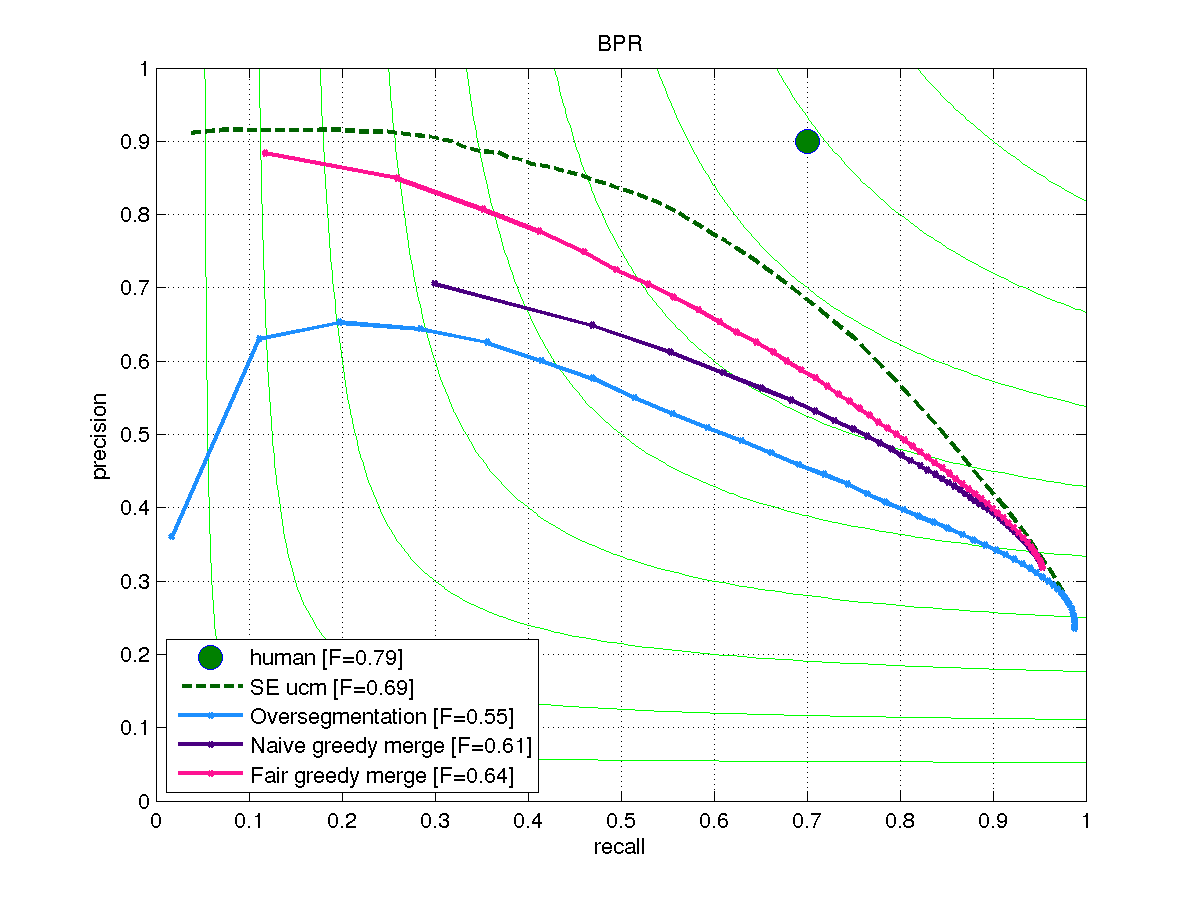
\includegraphics[width=0.7\textwidth]{images/plots/segs-to-greedy-merge-RIMC-BPR.png}
 }
 \subfigure[VPR]{%
  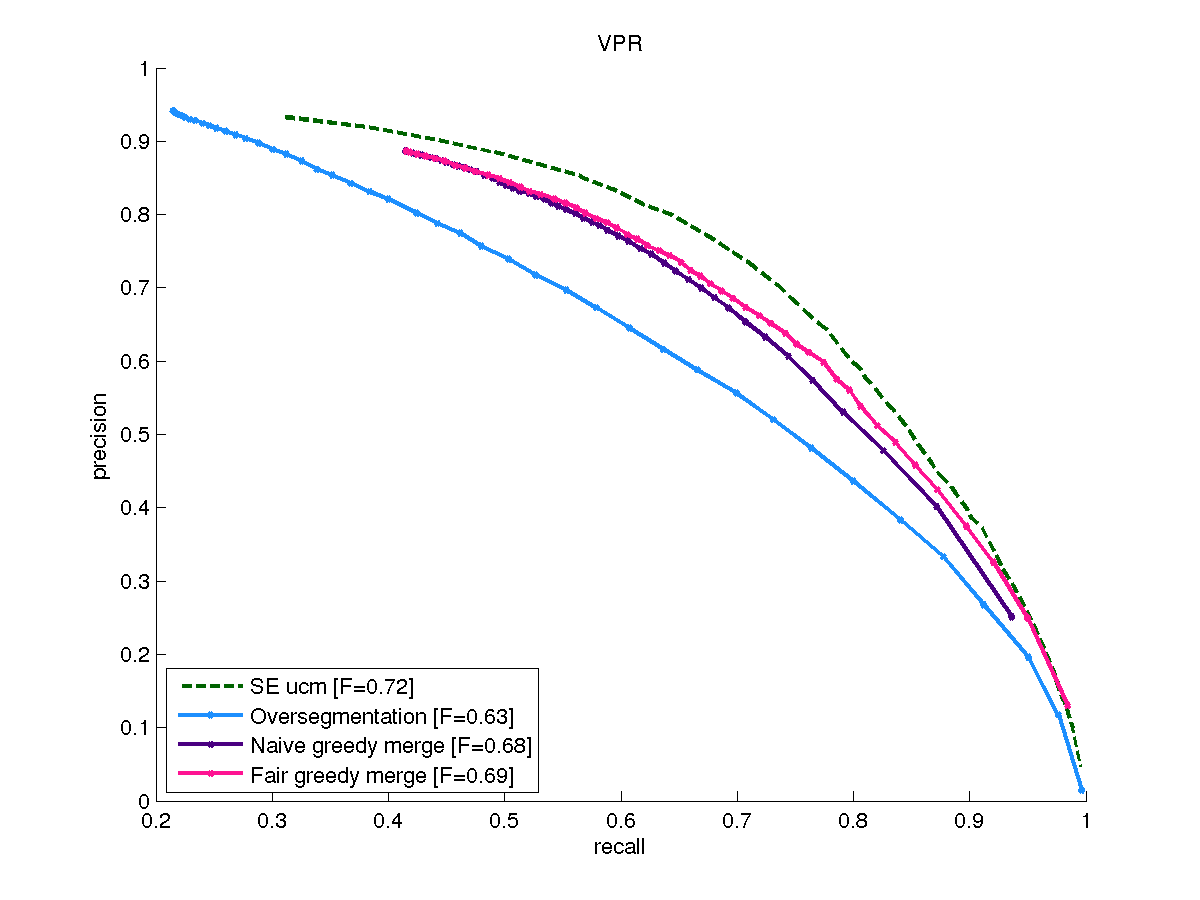
\includegraphics[width=0.7\textwidth]{images/plots/segs-to-greedy-merge-RIMC-VPR.png}
  %\label{fig:subfigure1}
 }
\caption{Greedy merge experiments. In all cases the scoring function used for patches comparison was the RIMC~(\hyperref[RIMC-maths]{RIMC description in Chapter 4}).} % \ref{RIMC-maths}
\label{fig:segs-to-greedy-merge-RIMC}
\end{figure}

\item{\bf Watershed region boundary:} We would like our watershed weighting strategy to take into account fine changes in the shape of the region boundary. To this end, we transform the watershed patch to contain exclusively the part of the watershed on which we are to cast our vote, and discard all other region boundaries present in the patch.

This approach does not guarantee closed contours - the part of the region boundary present in the patch would often be \textbf{just an image edge}. So we cannot use as a scoring function a region metric but must instead use a boundary-based one. We must, therefore, transform the segmentation patch from the tree leaf to a boundary patch. It is trivial~\cite{Arbelaez11} to obtain an edge map, given a segmentation. our transformed tree leaf patch is a binary edge map. As a scoring function we use the our boundary-based evaluation metric - BPR.

% BPR on contours - watershed arc and region boundary
Our conclusion from this experiment is that the combination of only the edge with the BPR provides poor means of judging the evidence of boundary in the leaves of the structured forest. Watershed region boundary is a very brittle cue. Further, BPR is parametrised on the pixel distance for which a match between the two segmentation boundaries is to be made. There is not a generic way to correctly choose such a distance for all forest segmentation patches and watershed locations. Accurate localisation of boundaries seems to be crucial for this weighting strategy, and this is not the case with the leaf segmentations and the watershed.

\item{\bf Oracle:} To evaluate the correctness of our weighting strategies, we've implemented an oracle for our pipeline. The question we wanted to answer is ``how well could we perform segmentation in the presence of perfect information?'' Our Structured voting lends itself easily to such an experiment using the ground truth segmentation. When scoring a given pixel on the watershed regions boundary, we use a ground truth segmentation patch, rather than the most likely segmentation learnt by the structured forest. The second patch, as in the regular experiments, is taken from the same pixel location in the watershed locations image.

\item{\bf Hardest negative mining:} Help determine where the voting fails the most. Conclusion: with so few votes per location, our approach would need much better leaves. We observed a lack of strong agreement in the leaves of the decision forest. The medoid segmentation patch, which is the only one casting a vote, is not necessarily representative of the set of segmentations that reached the leaf node of the tree.
% TODO figure of decision forest leaf, pref. different leaves

\item{\bf Line fitting:}
Our best performing weighting strategy. We implemented three line fitting algorithms:
\begin{enumerate}
  \item parametric, based on the derivative direction of the end-lines of the watershed edge we vote on,
  \item as above, but enforcing adherence to the centre of the image patch,
  \item linear least squares fitting to all the watershed edge pixels.
 % also possible - PCA-based fit
\end{enumerate}

Discuss performance \wrt different scoring functions. Notable that all 3 types of scoring functions - VPR, RI, BPR perform reasonably well with this watershed transformation. Normalisation of VPR. Asymmetry of normalisation and how it affects us.

\item{\bf Quadratic fitting:} % conic n=2; Polynomial
Conic sections - parabola, hyperbola and ellipse that fit the data. Too complex a model, thwarted by degenerate cases (best fitting parameters yield a 3-dimensional surface that doesn't intersect the $Z=0$ plane).

\item{\bf Voting scope:}
  \begin{itemize}
    \item{\bf Degraded baseline SE-UCM:} Have the SF output a pixel, or a $2\times2$, $4\times4$, $8\times8$ patch.
    \item{\bf Reduced vote scope:} This series of experiments aims at proving that casting a vote on a larger area is desireable, by doing exactly the opposite. We cast just $T$ votes ($T$ - number of trees in the decision forest) on a single pixel of the watershed location. As expected, that severely diminishes performance (\wrt averaging on the region boundary) since the voting scope is decreased to 1 pixel. Excessive localisation therefore hinders performance.
  \end{itemize}
Discussion: It would be useful to see the effect of a ``mixed'' scope of voting - cast vote on the whole region boundary, but use subdivided region boundary - the watershed arc in order to do the patch transformation.
\end{enumerate}

Important conclusions of the experiments:
\begin{enumerate}
 \item both watershed transformations and scoring functions are important,
 % \item scoring functions matter,
 \item a suitable %smart
 watershed transformation could greatly aid a ``weaker'' scoring function (\eg the benefit of greedy merge when using RI scoring function),
 \item our best watershed transformation has reasonable performance with all the scoring functions tried,
 \item oracle confirms the ranking of our experiments,
 \item simpler models work better for transforming the watershed patch (\eg quadratic and polynomial fitting are the worst performing experiments regardless of the scoring function used),
 \item voting scope is very important; a decrease in the voting scope seriously damages results; successfully increasing the voting scope is not trivial.
\end{enumerate}